

\setcounter{section}{4}
\section{Electrical Design}
\bigskip

\subsection{Power Management}
\medskip

Power consumption will be an important aspect to focus on because the ID Tags are a wearable electronic device, therefore, the device battery has to maintain charge over very long periods of time. One of the restrictions that must be considered is related to the size of the ID Tags; if an employee must wear their ID tag over long periods of time, as would be expected by users of this system, a large and heavy ID Tag is not an option. During prototype phase of the development stage, a 5V rechargeable lithium ion battery at 4000mAh will provide sufficient in power delivery and size for the ID tags. 

\bigskip
The ESP32 chip is a Dual-Core 32-bit microprocessor along with 448 KB of ROM, 520 KB of SRAM and 4MB of Flash memory. It also contains WiFi module, Bluetooth Module, Cryptographic Accelerator (a co-processor designed specifically to perform cryptographic operations), the RTC module, and other peripherals as shown in figure \ref{a_mode} \cite{R5-1-1}. In the normal active mode of operation where the ESP is sending and receiving data, the power consumption requires between 160-260mA. Under the assumption that the ESP is on and transmitting at all times and with a 5V, 4000mAH battery, the ID Tag device can achieve a lifetime of only 15 hours as calculated in the equation below.

\medskip
\begin{equation}
Battery Life Time = 4000mAH/260mA = 15.38 Hours
\end{equation}

\medskip
\begin{figure}[H]
\centering
    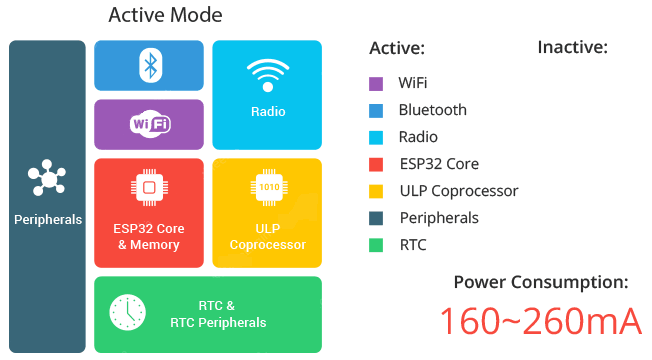
\includegraphics[scale=0.7]{./images/active_mode.png}
    \caption{ESP32 Active Mode Power Usage}
    \label{a_mode}
\end{figure}

\pagebreak
To optimize the battery life time when not under emergency mode, the ESP32 has an advanced power saving mode called Deep Sleep. Power consumption for ID tags can be cut back power usage by leveraging one of ESP32’s Sleep Modes and dramatically extending the battery life. In deep sleep mode, the CPU, most of the RAM and all the digital peripherals are powered off. The only parts of the chip that remains powered on are: RTC controller, RTC peripherals (including ULP co-processor), and RTC memories (slow and fast) as shown in figure \ref{ds_mode} \cite{R5-1-1}. The chip consumes around 10\(\mu\)A under deep sleep mode and using calculation shown in equation (2) the battery life time can be extended up to 400,000 hours.
\medskip
\begin{equation}
Battery Life Time = 4000mAH/10uA = 400,000 Hours
\end{equation}

\medskip
\begin{figure}[H]
\centering
    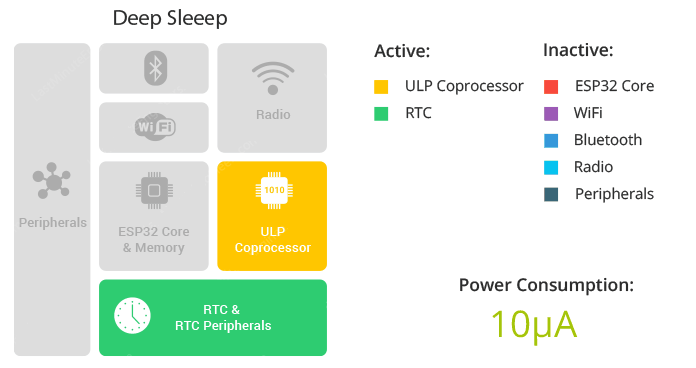
\includegraphics[scale=0.7]{./images/ds_mode.png}
    \caption{ESP32 Deep Sleep Mode Power Usage}
    \label{ds_mode}
\end{figure}

\bigskip
Developing a product that operates in emergency and disaster situations means that each component will have to operate in an extremely wide range of conditions. For this reason, each component of the system will include a backup power supply. Since size is not as much of a constraint for the beacons and data processing unit components of the system, it is easier to be more liberal with the size of the backup battery. The beacons and data processing unit is allowed an additional 9V 4000mAH rechargeable lithium ion battery backup. 


\pagebreak
\subsection{RF Harvester}
\medskip
Radio Frequency is an abundant source for energy harvesting especially in a radio wave rich environment. When Radio Waves reach an antenna it causes a changing potential difference across the antenna. The potential difference causes charge carriers to move along the length of the antenna in an attempt to equalize the field, and the RF-to-DC integrated circuit (Figure \ref{rf_bd}) is able to capture energy from the movement of those charge carriers. The energy is stored temporarily in a capacitor and then used to create a desired potential difference at the load \cite{R5-2-1}.

\medskip
\begin{figure}[H]
\centering
    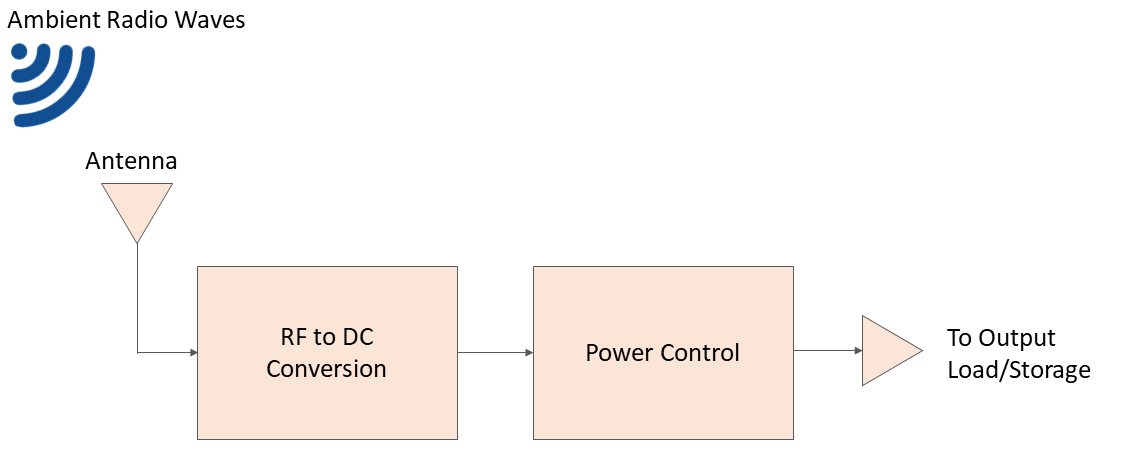
\includegraphics[scale=0.55]{./images/RF_H.png}
    \caption{RF Harvester Block Diagram}
    \label{rf_bd}
\end{figure}

There will be a demonstrable RF harvester circuit similar to Figure \ref{rf_c} that would convert ambient radio signal to DC voltage to charge the ID tag under deep sleep mode. During initial testing, the harvesting was able to collect up to 100 mV, however the ESP32 deep sleep mode requires 10 uA. Load calculation and capacitance optimization will need to be performed to further improve the reliability of the harvester. Once RF harvester test circuit produces adequate results in the prototype phase, the circuit will be implemented onto the ID Tag devices as PCB components. The RF harvester circuit designed for charging the ID tags will be collecting ambient RF power created from Wi-Fi and cellular communications to maintain charge for ESP32 during deep sleep mode.

\medskip
\begin{figure}[H]
\centering
    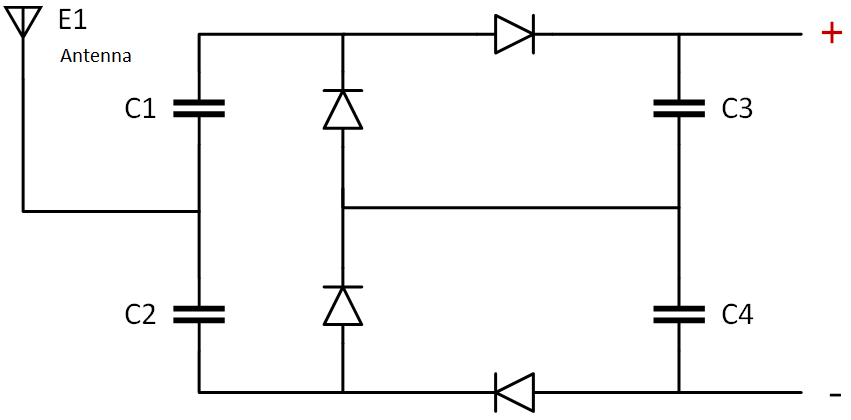
\includegraphics[scale=0.5]{./images/rf_circuit.png}
    \caption{RF Harvester Circuit Diagram}
    \label{rf_c}
\end{figure}

\pagebreak
\subsection{Electrical Design Specification}
\medskip
The system is designed for emergency disaster situations, it is crucial that sucient power is provided to each device at any given time. In order for the system to be reliable and, the electrical systems must be robust and efficient. TRIWAVE SYSTEMS has compiled a strict set of electrical requirements that ensures the beacons and ID tags will operate in a safe and efficient way.
\medskip
\bgroup
\def\arraystretch{1.5}
\begin{table}[H]
\centering
\begin{tabular}{ | m{3cm} | m{12.5cm} |}
\hline
\textbf{REQ.EC.1 - C} &  Each beacon shall be powered through standard North American power outlets (120V AC, 60Hz, type A/B)\\
\hline
\textbf{REQ.EC.2 - C} &  The Data Processing Unit (DPU) will be powered over USB by the device that it is plugged in to\\
\hline
\textbf{REQ.EC.3 - P} &  The ID tags must have a manual switch to toggle power on \\
\hline
\textbf{REQ.EC.4 - P} &  The ID Tags must be powered by 4.5V rechargeable lithium ion battery\\
\hline
\textbf{REQ.EC.5 - P} &  The ID tags must be under deep sleep mode drawing no more than 10 uA when not in emergency mode\\
\hline
\textbf{REQ.EC.6 - F} &  The beacons must use rechargeable 9V lithium battery as a backup power supply\\
\hline
\end{tabular}
\caption{Electrical Design Specification}
\end{table}
